\documentclass[11pt]{article}

\usepackage[T1]{fontenc} % extended font encoding
\usepackage{enumerate} % lists
\renewcommand{\familydefault}{\sfdefault} % sans-serif
\usepackage{microtype} % better text justification
\usepackage{graphicx} % allow including pictures
\usepackage{color} % colors for pictures
\usepackage{textcomp} % for textminus
\usepackage{pagecolor} % background color for the first page
\usepackage{afterpage} % ditto ^^
\usepackage[a4paper, landscape, margin=1.5cm]{geometry} % basic geometry
\fboxsep=5mm % minibox spacing
\pagenumbering{gobble} % disable page numbering

% Style for a simple numbered list
\newenvironment{packed_enumerate}{
\begin{enumerate}
  \setlength{\itemsep}{1pt}
  \setlength{\parskip}{0pt}
  \setlength{\parsep}{0pt}
}{\end{enumerate}}

% Style for a roman literal numbered list
\newenvironment{packed_enumerate_i}{
\begin{enumerate}[I]
  \setlength{\itemsep}{1pt}
  \setlength{\parskip}{0pt}
  \setlength{\parsep}{0pt}
}{\end{enumerate}}


% Metadata
\pdfinfo{
   /Author (Zlosynth Instruments)
   /Title  (Kaseta - User Manual)
}

\begin{document}

\pagecolor{black}\afterpage{\nopagecolor}

\title{\textcolor{white}{MANUAL}}
\author{}
\date{}

% Left column
\begin{minipage}{0.4\textwidth}
\color{white}
\maketitle

% Overview
\noindent\colorbox{white}
{
\begin{minipage}{0.85\textwidth}\color{black}
What it is. Inspired by tape machines. Achordion allows you to do many things, but in essence, it is just a bunch of oscillators that never go out of tune or out of scale! Apart from playing anything between lush pads and hellish walls of sound, it enables you to easily jam with other musicians and explore characters of different scales.
\end{minipage}
}

\vspace{1cm}

% Specs
\begin{minipage}{0.8\textwidth}\color{white}
\begin{tabular}{@{}rl@{}}
  Width & 20 HP \\
  Depth & 28 mm \\
  % TODO: Needs to be re-measured
  Power & +12 V (85 mA), \textminus12 V (7 mA) \\
  Input impedance & 100 kΩ \\
  CV inputs & \textminus5 to +5 V, 16-bit, 2 kHz \\
  Trigger output & 0 to +5 V, 10 ms \\
  Audio & 24-bit, 48 kHz
\end{tabular}
\end{minipage}

\vspace{1cm}

% Features
\begin{minipage}{0.8\textwidth}\color{white}
\begin{tabular}{@{}l}
  - Saturation \\
  - Compression \\
  - Harsh overdrive \\
  - Feedback designer \\
  - Granular synthesis \\
  - Four free-moving heads \\
  - Tone contol \\
  - Trigger sequencer \\
  - Oscillator \\
  - Rewind/speed simulation
\end{tabular}
\end{minipage}

\end{minipage}%
% Right column
\begin{minipage}{0.6\textwidth}
\vspace{8mm}
\begin{center}
  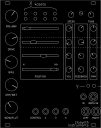
\includegraphics[width=1.0\textwidth]{schema.pdf}
\end{center}
\end{minipage}

\newpage
\color{black}



% Left column
\begin{minipage}[t]{0.35\textwidth}

\section {Warranty}

Bla bla.

\section{Installation}

Achordion is 20 HP wide. It is powered by a +12V/-12V 2x5 connector. The red stripe (-12V) must be connected on the side of the board marked with the white line. The module must be mounted in a Eurorack case.

\end{minipage}%
\begin{minipage}{0.05\textwidth}
\phantom{ }
\end{minipage}%
% Right column
\begin{minipage}[t]{0.55\textwidth}

\section{Controls, inputs and outputs}

Pre-amp
Tone
Saturation/drive
Bias
Wow
Flutter
Delay length
Head position
Head playback
Head feedback
Head pan

What is each pot doing.

How is the display used.

What is the button for.

How are delay heads grouped.

How to use CV input.

\end{minipage}

\newpage

\section{Pre-amp}

What is the range. What is it good for. What signalizes clipping.

Nothing plugged in, use tone as amp, some other as frequency control, play sine on input.

\section{Saturation}

About the maths behind, what it does on real tape.

Image of what happens to the sound.

Explanation of bias.

Explanation of the sweet spot with pre-amp.

Bias is most pronounced on weak input signal without distortion.

Danger zone.

\section{Delay}

Heads. Feedback vs blend. Ranges. Clock in. Gate out.

Longest delay is. Switchable ranges.

Image illusatration of the signal flow.

Switch to make volume a chance for the gate.

Tap-in, regular or clock signal in mapped control.

Image 

How to recover from feedback loop.

\section{Tone}

Images with low-pass, all-pass, high-pass positions.

Explanation on how it is applied per head.

Mention of the switch setting it for feedback/all.

\section{Wow and flutter}

Wow: Oscillation or change in pitch, caused by warped tape, low frequency, <4Hz

Flutter: Simulates scratched tape or friction, causes inconsistent information, vibration in frequency spectrum, high frequency, >4Hz

\section{Compression}

Explanation of what happens with output (saturation). Also can enable compression instead, using switch.

\section{Options}

Delay echo vs. audio rate
Quantization 1/8
Quantization 1/6
Wow cyclic vs. random
Flutter cyclic vs. random
Danger zone
Rewind/speed

\newpage

\section{Patch book}

Some basic combinations to get you started. TODO: Custom wow/flutter using position modulation.

\vspace{5mm}
\noindent
\begin{minipage}[t]{0.45\textwidth}

\subsection{Warm saturation}

\vspace{5mm}
\begin{center}
  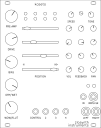
\includegraphics[width=0.7\textwidth]{schema-inverted.pdf}
\end{center}

* Basic hysteresis.
* Warm soft saturation on piano is nice.

\end{minipage}%
\begin{minipage}{0.05\textwidth}
\phantom{ }
\end{minipage}%
% Right column
\begin{minipage}[t]{0.45\textwidth}
\subsection{Wow and flutter}

\vspace{5mm}
\begin{center}
  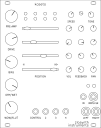
\includegraphics[width=0.7\textwidth]{schema-inverted.pdf}
\end{center}

Find a better name.

* Basic flutter with disabled hysteresis.
\end{minipage}

\newpage


\subsection{Simple echo}

* Basic evenly spread one time delay.

\subsection{Feedback pads}

* Basic feedback delay. Single head, slightly delayed.

\subsection{Comb filter}

* Audio level delay. Just one slightly delayed head playing and feeding back.
  Perhaps on specific tones.

\subsection{Thickiening of basic sine}

* Plain sine. All four heads playing in a small distance from each other.
  Producing reverb. Add flutter to make it forever moving and changing.

\subsection{Tremolo}

* Basic tremolo, just cyclic flutter.

\subsection{Rhytmical echo}

* Delays comming back, with some heads close, some far to repeat way later.

\subsection{Rhythm sequencer}

* Percussion rhythm.

\subsection{Almost sidechaining}

* When bass drum and single oscillator tone play at the same time with high
  saturation and low bias, it works like sidechaining.

\subsection{Cutting cymbals}

* Short cybmals, low bias cuts weak signal.

\subsection{Ping pong echo}

* Ping pong snare. Like Daughter's New Ways.

\subsection{Samples from the past}

* With non-warping delay, CV S and H input to delay value, selecting samples from
  the past.

\subsection{Rewind}

* Playing a mellow song, slow speed. Fading when approaching end, switch to another head.

\subsection{Distortion unchained}

* Hardcore distortion

\newpage





\noindent
\begin{minipage}[t]{0.3\textwidth}
\section{Configuration}
\end{minipage}%
\begin{minipage}{0.05\textwidth}
\phantom{ }
\end{minipage}%
% Center column
\begin{minipage}[t]{0.3\textwidth}
\section{Changelog}
\end{minipage}
\begin{minipage}{0.05\textwidth}
\phantom{ }
\end{minipage}%
% Right column
\begin{minipage}[t]{0.3\textwidth}
\section{Questions?}

\begin{center}
petr@zlosynth.com
\end{center}
\end{minipage}

\end{document}
